% Created 2021-01-24 Sun 22:49
% Intended LaTeX compiler: pdflatex
\documentclass[11pt]{article}
\usepackage[utf8]{inputenc}
\usepackage[T1]{fontenc}
\usepackage{graphicx}
\usepackage{grffile}
\usepackage{longtable}
\usepackage{wrapfig}
\usepackage{rotating}
\usepackage[normalem]{ulem}
\usepackage{amsmath}
\usepackage{textcomp}
\usepackage{amssymb}
\usepackage{capt-of}
\usepackage{hyperref}
\usepackage{minted}
\hypersetup{colorlinks=true, linkcolor=black, filecolor=red, urlcolor=blue}
\usepackage[turkish]{babel}
\author{Eren Hatırnaz}
\date{16 Aralık 2019}
\title{Yazılım Gündemi - 22\\\medskip
\large 16-22 Aralık 2019}
\hypersetup{
 pdfauthor={Eren Hatırnaz},
 pdftitle={Yazılım Gündemi - 22},
 pdfkeywords={},
 pdfsubject={},
 pdfcreator={Emacs 27.1 (Org mode 9.3)},
 pdflang={Turkish}}
\begin{document}

\maketitle
\tableofcontents \clearpage\shorthandoff{=}

\begin{center}
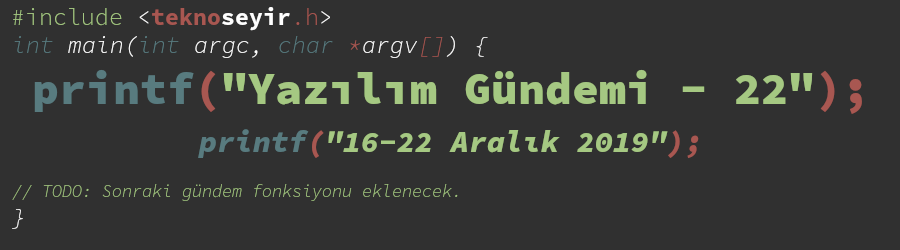
\includegraphics[width=.9\linewidth]{gorseller/yazilim-gundemi-banner.png}
\end{center}

\begin{center}
\href{../21/yazilim-gundemi-21.pdf}{< Önceki Gündem} | \textbf{16-22 Aralık 2019} | \href{../23/yazilim-gundemi-23.pdf}{Sonraki Gündem >}

\href{https://teknoseyir.com/blog/yazilim-gundemi-22-16-22-aralik-2019}{TeknoSeyir'de Oku}
\end{center}

\section{\href{https://visualstudiomagazine.com/articles/2019/12/17/net-5-next.aspx}{.NET 5 için yol haritası} açıklandı}
\label{sec:org3cf9aae}
.NET Framework çoğumuzun da bildiği gibi Microsoft'un çok uzun zamandır
geliştirmekte olduğu, tüm ekosistemini üzerine kurduğu bir uygulama çatısıydı.
.NET Core ise son 3-4 yıldır geliştirilmekte olan açık kaynak,
platformlar-arası (cross-platform) çalışabilen ve modern bir yapıya sahip
uygulama çatısı. Yazılım dünyasında değişen trendlerle birlikte ortama ayak
uyduran Microsoft, özellikle CEO olarak Satya Nadella'nın gelmesinden sonra
açık kaynak camiasına ve kendisinden pek beklenmeyecek hamleler de yaptı. İşte
.NET Core'da bu yeni anlayışın bir ürünü. Visual Studio Magazine dergisinin
internet sitesinde bu hafta yayınlanan bir yazıyla birlikte daha önce \href{https://news.microsoft.com/build2019/}{Build
2019} etkinliğinde duyurulan .NET 5 yol haritası da özetlenmiş oldu. O etkinlik
yazılım gündemi yazıları yazmaya başlamadan önceki bir tarihe denk geldiği için
bu yazıyı fırsat bilerek gündeme almak istedim.

\begin{center}
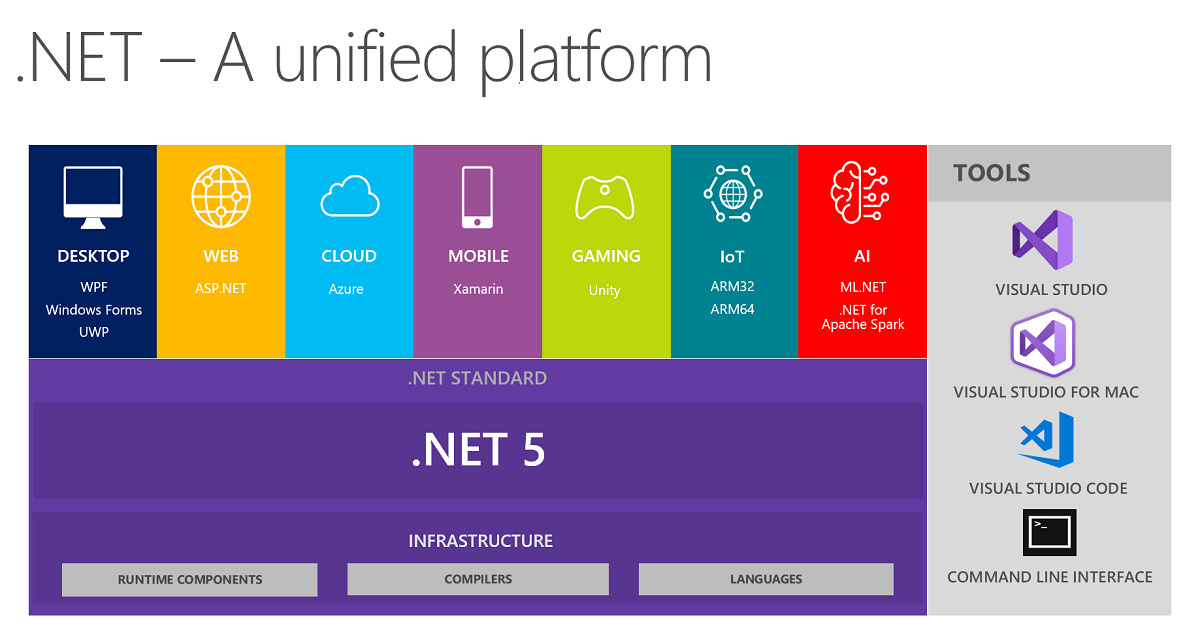
\includegraphics[width=.9\linewidth]{gorseller/dotnet5_platform.png}
\end{center}

Bildiğiniz tüm .NET'leri unutun! Bundan sonra tek bir .NET olacak, o da: .NET 5
(Biraz reklam metini gibi oldu ama :)). Microsoft'un tüm uygulama geliştirme
çözümleri (.NET Framework, .NET Core ve Xamarin/Mono) tek bir isim altında
birleşiyor ama bu sefer ne "Framework" ne de "Core" gibi ek kelimeler olacak;
sadece ".NET 5". 2020'nin ilk yarısı Preview sürümünün yayınlanması bekleniyor.

Önceki yazılım gündemlerinden birinde (bkz: \href{../14/yazilim-gundemi-14.pdf}{Yazılım Gündemi - 14}),
Microsoft'un, .NET Framework API'lerinin .NET Core projesine aktarılmasının
tamamlandığını duyurmuştu. O haberden Microsoft'un yöneliminin .NET Core
üzerinden devam etmek üzerine olduğunu anlamıştık zaten ve işte bugün de
kendimizi doğrulamış oluyoruz. .NET, eski kapalı-kaynak, sahipli, sadece
Windows'da çalışan kabuğundan sıyrılıyor ve yeni açık kaynak modern kimliğine
kavuşuyor.

\begin{center}
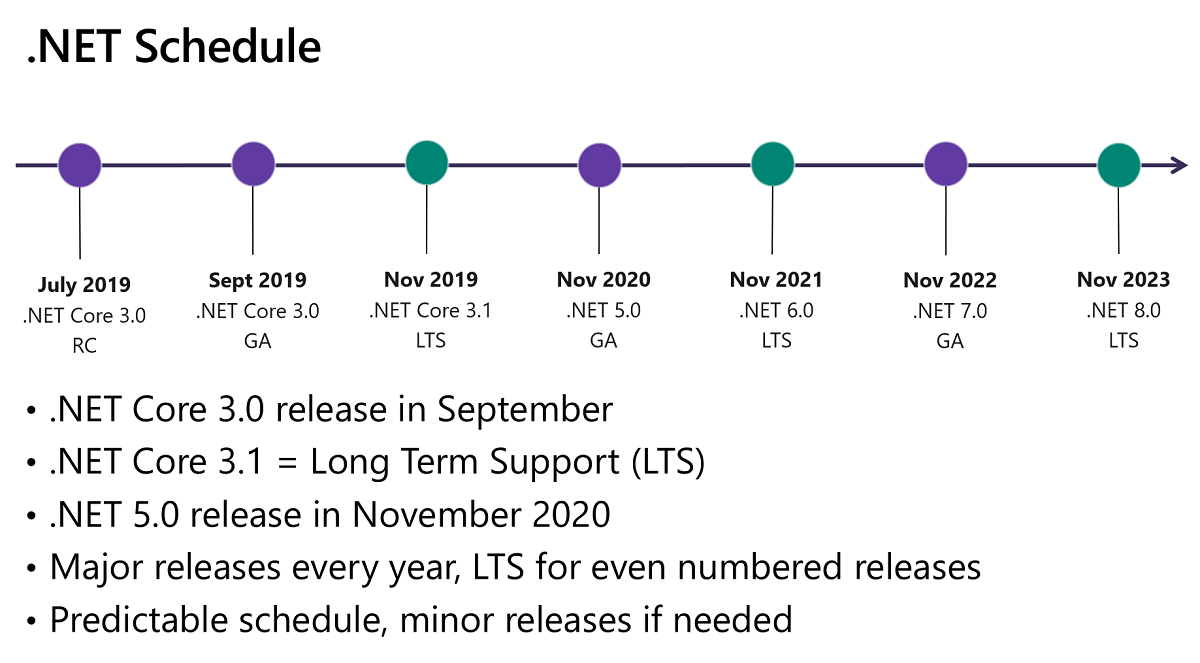
\includegraphics[width=.9\linewidth]{gorseller/dotnet_schedule.png}
\end{center}

.NET 5 sürümünün herkes tarafından erişilebilir (General Available) ilk sürümü
Kasım 2020 tarihinde duyurulması planlanıyor. Planlanan takvime göre uzun-dönem
desteklenecek (LTS - Long-term support) sürümler sadece tek sayılı yılların
Kasım ayında yayınlanacak ve 3 yıl boyunca desteklenmeye devam edecek. .NET 5
sürümünün geliştirilmesini takip etmek isterseniz \href{https://github.com/dotnet/corefx/milestone/44}{bu GitHub sayfasını} ziyaret
edebilirsiniz.
\section{Ruby 3.0 ile argüman işleme sistemi \href{https://www.ruby-lang.org/en/news/2019/12/12/separation-of-positional-and-keyword-arguments-in-ruby-3-0/}{değişecek}}
\label{sec:org5e805ec}
Bu haber aslında geçtiğimiz haftanın konusu ama geçtiğimiz hafta gündemi biraz
geç yayınlamak durumunda olduğum için bu haberi bu haftaya ertelemiştim. Bir
programlama dili ile ilgili önemli sayılabilecek bir değişiklik olduğu için
haberi atlamak da istemedim. Ruby programlama dilinin 3.0 numaralı sürümünde
bizi geriye uyumluluğu olmayan bir takım temel değişiklikler bekliyor.

Başka birkaç programlama dilinde de olduğu gibi Ruby dilinde de pozisyonel
(positional) ve anahtar kelime (keyword) argümanları mevcut. Örnek üzerinden
anlatmak gerekirse:
\begin{minted}[breaklines=true,breakanywhere=true,frame=lines, linenos, label=Ruby, labelposition=topline]{ruby}
def foo(k: 14)
  puts k
end

h = { k: 24 }

foo(h)
\end{minted}
Bu kod parçasındaki \texttt{foo} fonksiyonunda argüman keyword şeklinde tanımlanmış.
Yani argümanın bir ismi var ve o argümana bir değer verilmediği zaman
alabileceği bir varsayılan değeri var. Sonrasında ise \texttt{h} isimli \emph{Hash}
tipinde bir değişken tanımladık ve onu \texttt{foo} fonksiyonuna positional argüman
olarak gönderdik. Bu durumda Ruby 2.7, positional olarak gönderilen argümanı
alıp keywork şeklinde gönderiyor fonksiyona yani sorunsuz çalışıyor ama artık
Ruby 2.7 bu kod parçası için \textbf{Warning} göstermeye başlayacak çünkü bu otomatik
dönüştürme işlemi artık deprecate oldu ve Ruby 3.0'da bu kod parçası
çalışmayacak, \textbf{ArgumentError} hatası verecek.
\begin{minted}[breaklines=true,breakanywhere=true,frame=lines, linenos, label=Ruby, labelposition=topline]{ruby}
def bar(h, **kwargs)
  puts h
end

bar(k: 42)
\end{minted}
Bu kod parçasındaki \texttt{bar} fonksiyonu ise argümanlar bir positional ve bir
keyword şeklinde tanımlanmış. Sonrasında ise \texttt{bar} fonksiyonuna keyword
şeklinde bir argüman göndermişiz. Bu kod parçası da Ruby 2.7'de, keyword'den
\emph{Hash} positional'a dönüştürülerek çalışıyor, tabii ki yine \textbf{Warning}
göstererek. Aynı şekilde bu kod parçası da Ruby 3.0'da çalışmayacak ve
\textbf{ArgumentError} hatası verecek.

"Peki bu tarz bir kullanım senaryosuna ihtiyaç duyduğumuzda ne yapacağız?"
dediğinizi duyar gibiyim. Ruby geliştiricileri bu durumlarda kullanmak için şu
özellikleri eklediler:
\begin{minted}[breaklines=true,breakanywhere=true,frame=lines, linenos, label=Ruby, labelposition=topline]{ruby}
foo(**h)

bar({ k: 42 })
\end{minted}
Bu şekilde kullandığınızda yine eskisi gibi kodlarınız çalışmaya devam edecek.
Dediğim gibi her ne kadar birden bire desteği kesilmeyecek olsa bile bu
değişikliğe uygun olarak kodlarınızı düzenlemeniz gerekecektir. Aklınızda
bulunsun. Bu değişikliğin sebebi olarak ise keyword ve positional formattaki
argümanların, birbirlerine çevrildikleri için karışıklık yaratması. Ruby
3.0'da çevrilmeyecekler ve fonksiyonlar hangi formatta argüman alması için
kodlanmışsa o şekilde çalışacak.

Ayrıca bu hafta içerisinde Ruby'nin 2.7.0 Release Candidate 2 \href{https://www.ruby-lang.org/en/news/2019/12/21/2-7-0-rc2-released/}{sürümü de
duyuruldu}. Final sürümünün ise 25 Aralık günü yayınlanması planlanıyor.
Sanırım bir sonraki Yazılım Gündeminde "Ruby 2.7 ile gelen özellikler"i
konuşacağız.
\section{Eclipse 2019-12 \href{https://www.eclipse.org/eclipseide/2019-12/noteworthy/}{duyuruldu}}
\label{sec:org50e3367}
Her ne kadar genelde Java teknolojileri için kullanılsa da diğer birçok dil
için de desteği olan geliştirme ortamı Eclipse, bu yılın son büyük numaralı
sürümünü duyurdu. Yeni eklenen veya değişen çok fazla özellik var, hepsine
burada değinemem elbette ama birkaç tanesini aktarmak gerekirse:

\begin{center}
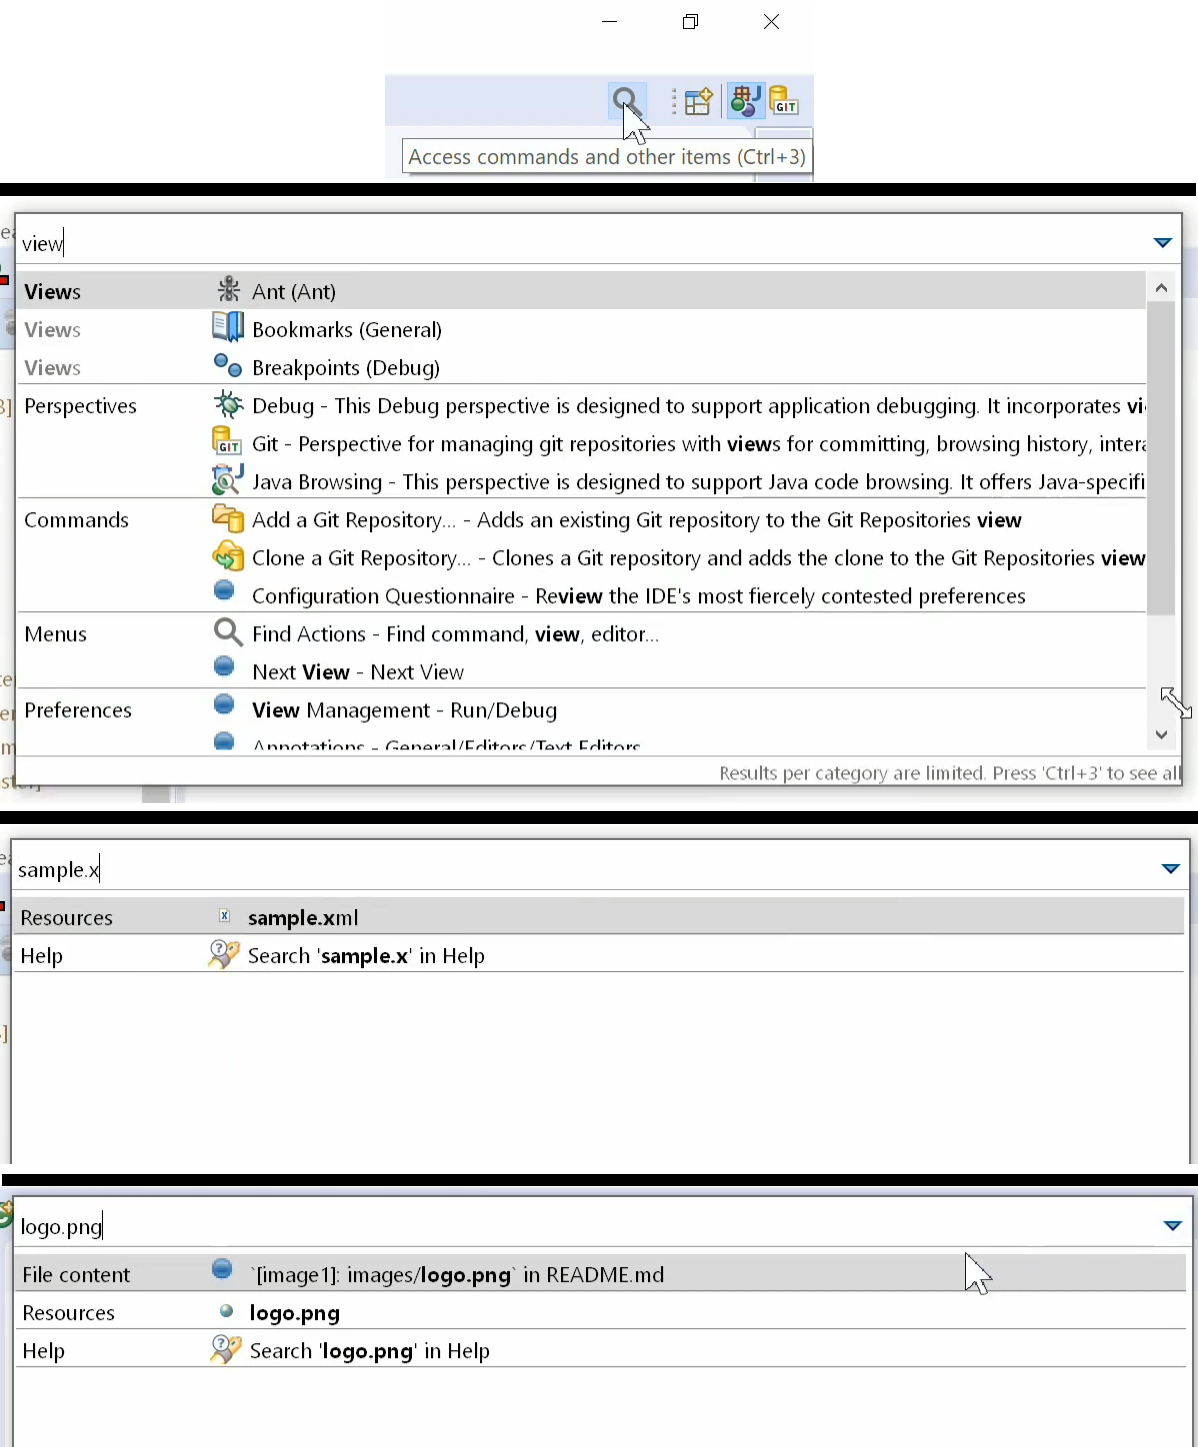
\includegraphics[width=.9\linewidth]{gorseller/eclipse1912-actions.png}
\end{center}

Diğer birkaç IDE ve metin editöründe de görmeye alıştığımız, tüm arama
işlemlerinin tek bir pencere ya da popup panel üzerinden halledildiği arama
özelliği sonunda Eclipse'ye de gelmiş. Artık aynı popup panel üzerinde hem
Eclipse komutlarını ("Build", "Build\&Run" vb. gibi menülerdeki her şey) hem de
proje içerisindeki dosya isimlerini ve dosyaların içeriklerinde arama
yapabileceğiz. Benim şahsen diğer IDE'lerde çok kullandığım bir özellik ve
Eclipse'ye gelmiş olmasına sevindim. Bu özelliği kullanmak için menü çubuğunun
hemen altındaki toolbarın en sağındaki kısımda bir büyüteç ikonu göreceksiniz
ona tıklarsanız bahsettiğim popup panel açılır ya da \textbf{CTRL + 3} kombinasyonlu
kısayolu tercih edebilirsiniz.

\begin{center}
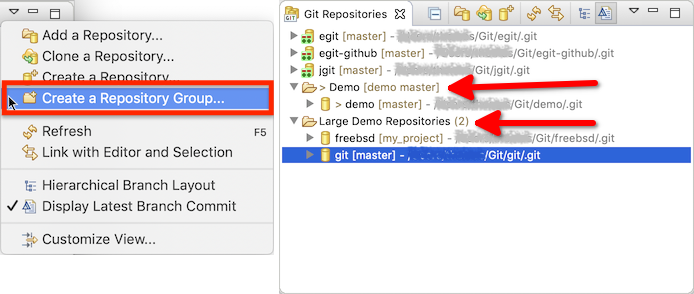
\includegraphics[width=.9\linewidth]{gorseller/eclipse1912-git-group.png}
\end{center}

Eclipse içerisinde aynı zamanda Git versiyon kontrol sistemi için entegre
araçlar takımları da mevcut. Bu sürümde ise Git Repositories kısmına
"Repository Group" özelliği geldi. İsminden de anlaşıldığı üzere birden çok git
deposunu tek bir grup altında göstermeye yarayan bir özellik.

\begin{center}
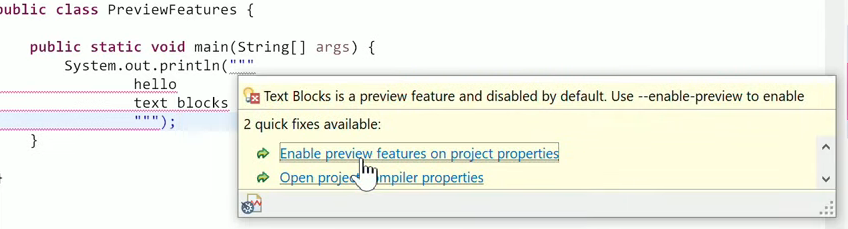
\includegraphics[width=.9\linewidth]{gorseller/eclipse1912-coklu-satir-string.png}
\end{center}

Bunların dışında java yetenekleri olarak da Java 13 ile birlikte gelen birçok
özelliğe destek veriyor. Java 13 (JDK 13) ile gelen bir özellikten \href{../03/yazilim-gundemi-03.pdf}{Yazılım
Gündemi - 3} yazısında bahsetmiştim. O yazıda bahsettiğim çok satırlı String
ifadeler özelliği artık Eclipse 2019-12'de destekleniyor. Yalnız bu özelliği
öncelikle aktifleştirmek gerekiyor. Bunun için yukarıdaki ekran görüntüsündeki
gibi bir kod yazıp, Quick Fix menüsünden ilgili özelliği aktifleştirebilir ya
da menülerden Project > Properties > Java Compiler altındaki "Enable preview
features for Java 13" yazısının yanındaki kutucuğu işaretleyerek aynı şekilde
özelliği açabilirsiniz.

Eclipse 2019-12 sürümüyle birlikte gelen diğer özellik ve değişiklikler için
konu başlığına eklediğim bağlantıya tıklayabilirsiniz.
\section{Jetbrains, \href{https://blog.jetbrains.com/idea/2019/12/intellij-platform-roadmap-for-2020/}{IntelliJ Platformu için 2020 yol haritası}nı açıkladı}
\label{sec:org1681686}
JetBrains, yazılım sektörü için çok iyi araçlar ve diller üreten bir firma.
Zaten yazılım sektörünün içinde olup ya da bu konulara ilgi duyup da JetBrains
araçlarının en az birini kullanmamış olan yoktur diye tahmin ediyorum. Bu hafta
içersinde de Java teknolojileri için geliştirdikleri IDE çözümü IntelliJ IDEA
ve IntelliJ Platform tabanlı diğer IDE'ler için 2020 yılı yol haritasını
açıkladılar. Yani bu yol haritası, Android Studio'yu da etkiliyor.

Yol haritasında öncelikli konu olarak "Performans" belirlenmiş. Geçtiğimiz yıl
boyunca IDE'nin açılma hızıyla ilgili \href{https://blog.jetbrains.com/idea/2019/10/preview-the-performance-improvements-in-intellij-idea-2019-3/}{birkaç iyileştirme yapmışlardı}.
Önümüzdeki yıl ise indexing işleminin performansıyla ilgili iyileştirmeler
üzerine çalışacaklarmış. IDE çalışırken gerek otomatik tamamlama özelliği için
gerekse de diğer ihtiyaçlardan dolayı indexing işlemi yapıyor. Bir projeyi
açarken en çok vakit alan kısım da zaten çoğunlukla bu oluyor. Bundan dolayı,
indexing verilerinin takımlardaki kişiler arasında paylaşılabilmesini sağlamaya
çalışacaklar. Yani bir proje sizin bilgisayarınızda indexlenmişse bunu başka
bir bilgisayardaki IntelliJ ile açtığınızda tekrar indexing'e gerek kalmayacak.
Bir de buna ek olarak bu indexing işlemi sırasında IDE'nin donmamasını
sağlayacak iyileştirmeler yapılacakmış. Yani projeyi açıp, indexing işleminin
bitmesini beklemek yerine kod yazmaya başlayabileceğiz ve indexing de
arkaplanda olmaya devam edecek. Projeyi açtıktan sonra IDE'nin kendine
gelmesini beklemek benim de pek sevmediğim bir durum o yüzden bu konudaki
iyileştirmelere şahsen muhtacım.

Yol haritasındaki bir diğer konu ise özellikle 2019 yılında popülerliği oldukça
artan "ortak düzenleme" (Collaborative Editing) konusu. Yani bir bilgisayarda
çalışan IDE'ye başka bir bilgisayar üzerinden bağlanılması ve ortak bir çalışma
ortamında kod yazılmasından bahsediyorum. Bu yönde çalışmaların devam ettiğini
belirtmişler ve özelliğin öncelikle Rider isimli IDE'ye geleceğini daha sonra
diğer IDE'lere de ekleneceğini belirtmişler ama bu özellik uzun soluklu bir
efor gerektirdiği için öyle 2020'nin hemen ilk aylarında beklemeyin diyorlar.

Açıklanan yol haritasında çok daha fazla konu mevcut fakat hepsinden burada
bahsedemem malumunuz eğer tüm yol haritası hakkında bilgi edinmek isterseniz
konu başlığına eklediğim bağlantıya tıklayabilirsiniz.
\section{\href{https://www.scala-lang.org/2019/12/18/road-to-scala-3.html}{Scala 3 için yol haritası} açıklandı}
\label{sec:orgb630e3c}
JVM platformu üzerinde geliştirilen Scala programlama dilinin 3. sürümü için
geliştirici takımı bir yol haritası yayınladı. Her ne kadar hiç deneyimim
olmadığı bir programlama dili olsa da gündeme çeşitlilik katması açısından bunu
da değerlendirmek istedim.

Öncelikle Scala 2.14 için çalışmayı bıraktıklarını ve o sürüm için planlanan
her şeyin Scala 3'e aktarıldığını belirtmişler. Aslında Scala 2.13'ü bir ara
geçiş sürümü olarak düşünmüşler ama sonrasında yaptıkları konuşmalardan sonra
buna gerek olmadığına karar vermişler ve doğrudan 3 numaralı sürüme yükselmeye
karar vermişler. İlk Release Candidate sürümünün 2020 yılı sonunda yayınlanması
planlanıyor. Yani daha bir yıl var diyebiliriz.

Yol haritası yazısı boyunca en çok vurgu yapılan konu ise geriye ve ileriye
uyumluluk mevzusu. Geriye uyumluluk (backwards compatibility) çok sık
duyduğumuz bir kavram fakat ileriye uyumluluğu (forwards compatibility) ben de
ilk kez duydum. Anladığım kadarıyla Scala 2.13 ve Scala 3 sürümleri hemen hemen
aynı kodları çalıştırabilecekler. Bu uyumluluğun sağlanabilmesi için de
standard library ismini verdiğimiz ana kütüphanede ekleme ve çıkarma
yapmayacaklarmış, sadece olan sınıflar üzerinde geliştirmeler yapılacakmış.
Fakat bu olay Scala 3.2 sürümüne kadar devam edecek, bu sürümden sonra ise
kendine ait bir standard library ile yola devam edilecek. Anladığım kadarıyla
Scala 3 bir geçiş sürümü olacak. Ayrıca Scala 2.13 sürümünde desteklenen macro
özelliği Scala 3'te farklı bir hal alıyor, yani bu özelliği kullanan bir
projeniz varsa o kısımları yeniden yazmak durumunda kalacaksınız.

Yol haritasındaki diğer detaylar için konu başlığına eklediğim bağlantıya
tıklayabilirsiniz. Yanlış değerlendirdiğim bir durum varsa lütfen yorumlar
bölümünde beni uyarın.
\section{Yaklaşan Etkinlikler}
\label{sec:org4e42179}
\begin{longtable}{|p{8cm}|l|l|}
\hline
Etkinlik İsmi & Yeri & Tarihi\\
\hline
\endfirsthead
\multicolumn{3}{l}{Önceki sayfadan devam ediyor} \\
\hline

Etkinlik İsmi & Yeri & Tarihi \\

\hline
\endhead
\hline\multicolumn{3}{r}{Devamı sonraki sayfada} \\
\endfoot
\endlastfoot
\hline
\href{https://kommunity.com/bilge-adam-teknoloji/events/postgresqlde-ileri-seviyede-performans-yonetimi}{PostgreSQL'de İleri Seviyede Performans Yönetimi} & Ankara & 24 Aralık 18:00\\
\href{https://kommunity.com/nsistanbul/events/nsistanbul-aralik-2019-bulusmasi}{NSIstanbul Aralık 2019 Buluşması} & İstanbul & 24 Aralık 19:30\\
\href{https://www.eventbrite.com/e/artrlms-gerceklik-platformlar-tickets-86102672411}{Artırılmış Gerçeklik Platformları} & Ankara & 25 Aralık 18:00\\
\href{https://www.eventbrite.com/e/codeyapkredi-vol-3-efsaneler-ve-gerceklerle-yapay-zeka-tickets-86411628507}{Code.YapıKredi Vol 3: Efsaneler ve Gerçeklerle Yapay Zeka} & İstanbul & 25 Aralık 19:00\\
\href{https://kommunity.com/sovos-foriba-rd/events/octopus-deploy-ile-cicd-surecleri}{Octopus Deploy ile CI/CD Süreçleri} & İstanbul & 26 Aralık 18:00\\
\href{https://kommunity.com/kodluyoruz/events/geldi-gelecek-teknoloji-sohbetleri-sertac-doganay-aykut-ibrisim}{Geldi Gelecek // Teknoloji Sohbetleri} & İstanbul & 26 Aralık 19:00\\
\href{https://kommunity.com/devnot-yazilimci-bulusmalari/events/machine-learning-day}{Machine Learning Day} & İstanbul & 28 Aralık 10:00\\
\href{https://www.meetup.com/tr-TR/Hukuk-ve-Teknoliji-Meetup-Grubu/events/267223619/}{KVKK ve GDPR Kapsamında Veri Güvenliği} & Ankara & 3 Ocak 18:30\\
\hline
\end{longtable}
\section{Diğer Haberler}
\label{sec:org287e31f}
\begin{itemize}
\item Finlandiya, online yapay zeka derslerini \href{https://www.elementsofai.com/}{ücretsiz olarak herkese açtı}.
Dersler burada: \href{https://www.elementsofai.com/}{Elements of AI}.
\item BMW, ürünlerinde kullandığı yapay zeka algoritmalarını \href{https://www.bmwblog.com/2019/12/13/bmw-shares-ai-algorithms-used-in-production-available-on-github/}{açık kaynak olarak
paylaştı}. \href{https://github.com/BMW-InnovationLab}{GitHub Deposu}
\item Standford Üniversitesi, \href{https://hai.stanford.edu/news/introducing-ai-index-2019-report}{Yapay Zeka İndeksi 2019 Raporu}nu yayınlandı.
\item GitHub, Actions özelliğinin Runner kısmını \href{https://github.blog/changelog/2019-12-19-github-actions-the-runner-is-now-open-sourced/}{açık kaynak hale getirdi}.
\item Ubisoft, C++ kullanıcı arayüzü kütüphanesi Dear ImGui'ye \href{https://montreal.ubisoft.com/en/ubisoft-sponsors-user-interface-library-for-c-dear-imgui/}{sponsor oldu}.
\href{https://github.com/ocornut/imgui}{GitHub Deposu}
\item IBM, Swift programlama diline \href{https://forums.swift.org/t/december-12th-2019/31735}{katkı yapmayı bırakıyor}.
\item Statik kod analizi aracı PVS-Studio, \href{https://www.viva64.com/en/b/0699/}{2019 yılında en çok karşılaşılan 10
Java hatası}nı tespit etti.
\item 8 yıllık bir Python 3 hatası bu hafta \href{https://bugs.python.org/issue13153}{giderildi}.
\item Visual Studio 2019 v16.4.2 \href{https://docs.microsoft.com/en-us/visualstudio/releases/2019/release-notes\#16.4.2}{sürümü yayınlandı}.
\item Google'ın açık kaynak olarak geliştirdiği JavaScript ve WebAssembly motoru
V8'in 8.0 \href{https://v8.dev/blog/v8-release-80}{sürümü duyuruldu}.
\item Redis'in v6.0 Release Candidate 1 \href{http://antirez.com/news/131}{sürümü yayınlandı}.
\item Rust programlama dilinin 1.40.0 \href{https://blog.rust-lang.org/2019/12/19/Rust-1.40.0.html}{sürümü duyuruldu}.
\item Crystal programlama dilinin 0.32.1 \href{https://crystal-lang.org/2019/12/18/crystal-0.32.1-released.html}{sürümü yayınlandı}.
\item EmberJS kütüphanesinin 3.15 "Octane" kod isimli \href{https://blog.emberjs.com/2019/12/20/ember-3-15-released.html}{sürümü yayınlandı}.
\item Google, memory-safe programlama dili \href{https://github.com/google/wuffs}{wuffs}'un 0.2.0 \href{https://groups.google.com/forum/m/\#!topic/wuffs/Ui9d3usmZNc}{sürümünü yayınladı}.
\item RethinkDB 2.4.0 sürümü \href{https://rethinkdb.com/blog/2.4.0-release}{duyuruldu}. \href{https://github.com/rethinkdb/rethinkdb/blob/v2.4.x/NOTES.md\#release-240-night-of-the-living-dead}{Sürüm Notları}
\item CMake 3.16.2 \href{https://blog.kitware.com/cmake-3-16-2-available-for-download/}{sürümü yayınlandı}.
\item \href{https://ionutbalosin.com/2019/12/jvm-garbage-collectors-benchmarks-report-19-12/}{JVM Garbace Collectors Benchmarks Raporu 19.12} yayınlandı.
\item C ile yazılmış PHP Framework sistemi Phalcon 4.0.0 \href{https://blog.phalcon.io/post/phalcon-4-0-0-released}{sürümünü duyurdu}.
\item PHP versiyonunuzdaki açıkları ve onları gideren patch'leri öğrenmenizi
sağlayan araç php-version-audio, 1.3.2 sürümünü \href{https://github.com/lightswitch05/php-version-audit/releases/tag/1.3.2}{duyurdu}.
\item Rust için http kütüphanesi Thruster, v0.8.0 \href{https://www.reddit.com/r/rust/comments/edss48/announcing\_thruster\_080\_stable\_asyncawait\_updated/}{sürümünü yayınladı}. \href{https://github.com/trezm/Thruster}{GitHub Deposu}
\end{itemize}
\section{Lisans}
\label{sec:org4fbf47a}
\begin{center}
\begin{center}

\includegraphics[height=1.5cm]{../../../img/CC_BY-NC-SA_4.0.png}
\end{center}

\href{yazilim-gundemi-22.pdf}{Yazılım Gündemi - 22} yazısı \href{https://erenhatirnaz.github.io}{Eren Hatırnaz} tarafından \href{http://creativecommons.org/licenses/by-nc-sa/4.0/}{Creative Commons
Atıf-GayriTicari-AynıLisanslaPaylaş 4.0 Uluslararası Lisansı} (CC BY-NC-SA 4.0)
ile lisanslanmıştır.
\end{center}
\end{document}
